\documentclass[border=3pt]{standalone}
% Shared preamble for the standalone figures of qurl_explained.tex.
% Build a figure from this folder:   tectonic fig_<name>.tex
% Colours: blue = full precision (FP), orange = 8-bit.
\usepackage[T1]{fontenc}
\usepackage{lmodern}
\usepackage{amsmath,amssymb}
\usepackage[dvipsnames]{xcolor}
\usepackage{tikz}
\usetikzlibrary{positioning,arrows.meta,calc,decorations.pathreplacing}
\usepackage{pgfplots}
\pgfplotsset{compat=1.17}
\colorlet{fp}{RoyalBlue}
\colorlet{qb}{BurntOrange}
\colorlet{good}{ForestGreen}
\colorlet{bad}{BrickRed}
\newcommand{\pold}{\pi_{\mathrm{old}}}
\newcommand{\thold}{\theta_{\mathrm{old}}}
\newcommand{\qthold}{\hat\theta_{\mathrm{old}}}
\tikzset{
  box/.style={draw, rounded corners=3pt, align=center, inner sep=4pt, font=\small},
  arr/.style={-{Stealth[length=2.2mm]}, thick},
  lab/.style={font=\footnotesize, align=center},
}
\pgfplotsset{
  small axes/.style={
    tick label style={font=\footnotesize}, label style={font=\footnotesize},
    title style={font=\small}, every axis plot/.append style={line join=round}},
}

\begin{document}
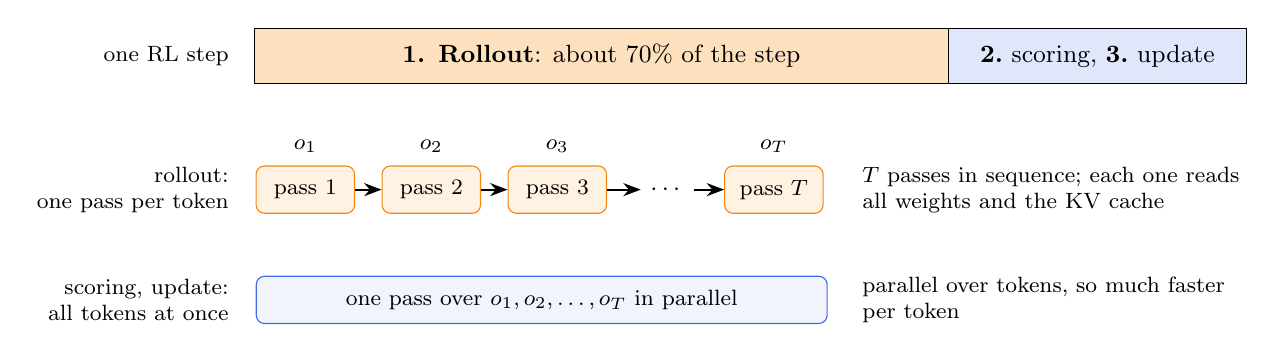
\begin{tikzpicture}[font=\small, tok/.style={box, minimum width=1.25cm, minimum height=0.6cm, inner sep=1pt, font=\footnotesize}]
\def\W{12.6}
% one RL step as a bar
\fill[qb!22] (0,0) rectangle (0.7*\W,0.7);
\fill[fp!16] (0.7*\W,0) rectangle (\W,0.7);
\draw (0,0) rectangle (\W,0.7);
\draw (0.7*\W,0) -- (0.7*\W,0.7);
\node at (0.35*\W,0.35) {\textbf{1. Rollout}: about 70\% of the step};
\node at (0.85*\W,0.35) {\textbf{2.}~scoring, \textbf{3.}~update};
\node[lab, anchor=east] at (-0.2,0.35) {one RL step};
% rollout: one forward pass per token
\def\ya{-1.35}
\node[lab, anchor=east, align=right] at (-0.2,\ya) {rollout:\\ one pass per token};
\foreach \i/\x in {1/0.65, 2/2.25, 3/3.85} {
  \node[tok, draw=qb, fill=qb!9] (p\i) at (\x,\ya) {pass \i};
  \node[font=\footnotesize, above=1pt of p\i] {$o_{\i}$};
}
\node (dots) at (5.25,\ya) {$\cdots$};
\node[tok, draw=qb, fill=qb!9] (pT) at (6.6,\ya) {pass $T$};
\node[font=\footnotesize, above=1pt of pT] {$o_T$};
\draw[arr] (p1) -- (p2); \draw[arr] (p2) -- (p3); \draw[arr] (p3) -- (dots); \draw[arr] (dots) -- (pT);
\node[lab, anchor=west, text width=4.9cm, align=left] at (7.6,\ya) {$T$ passes in sequence; each one reads all weights and the KV cache};
% scoring and update: all tokens at once
\def\yb{-2.75}
\node[lab, anchor=east, align=right] at (-0.2,\yb) {scoring, update:\\ all tokens at once};
\node[tok, draw=fp, fill=fp!7, minimum width=7.25cm, anchor=west] at (0.02,\yb) {one pass over $o_1,o_2,\dots,o_T$ in parallel};
\node[lab, anchor=west, text width=4.9cm, align=left] at (7.6,\yb) {parallel over tokens, so much faster per token};
\end{tikzpicture}
\end{document}
